\section{IEEE 802.15.4}\label{ss:IEEE802154}

Das ‚Institute of Electrical and Electronics Engineers‘ (IEEE) definiert in seinem Standard 802.15.4 Protokolle für ein ‚Low Data Rate - Wireless Personal Area Network‘ (LR-WPAN). Die Art der Geräte, die für eine solche Art von Netz verwendet werden sollen, ist dabei nicht genauer spezifiziert. Sinnvoll ist der Einsatz vor allem bei Systemen wie Sensoren, Lichtquellen oder Schaltern, bei welchen eine niedrige Datenrate vollkommen ausreicht um miteinander zu kommunizieren. Grundsätzlich ist die Verwendung des Standards auch bei höherwertigen Geräten wie z.B. Handys oder anderen Multimediageräten möglich, allerdings ist die Sinnhaftigkeit eines solchen Einsatzes fragwürdig, da in Hinsicht auf die geringe Datenübertragungsrate viele Übertragungs- und Kommunikationsfunktionen solcher Geräte wohl kaum realisierbar wären. \\
Zur Kommunikation mehrerer Teilnehmer in einem nach 802.15.4-standardisierten Netzes werden die o.g. Topologien ‚Stern‘ und ‚Peer-to-Peer‘ unterstützt. Sollte die Spezifikation ‚ZigBee‘,  welche den 802.15.4 Standard erweitert, verwendet werden, können darüber hinaus auch vermaschte Netze realisiert werden. \\
Der Standard sendet laut Definition festgelegtem Frequenzspektrum auf den lizenzfreien Frequenzen 868-868,8 MHz (Europa), 902-928 MHz (Nordamerika, Australien) oder 2400 bis 2483,5 MHz (weltweit). Um die Frequenzen darüber hinaus zu spreizen, wird ein ‚Direct Sequence Spread Spectrum‘-Verfahren (DSSS) verwendet.\\ 
Um den Zugriff auf das Medium untereinander zu koordinieren, wird CSMA/CA (‚Carrier Sense Multiple Access/Collision Avoidance‘) verwendet. Das bedeutet, dass, bevor ein Gerät mit einer Übertragung beginnt, überprüft wird, ob das Übertragungsmedium nicht bereits von einem anderen Endgerät genutzt wird. Ist das Medium nicht belegt, kann das Endgerät, welches das Medium überprüft hat, anfangen, seine Daten zu übertragen.\\
Der Standard erreicht Übertragungsraten zwischen 20 KB/s - 40 KB/s in den Frequenzbereichen von 868 MHz und 902-928 MHz, wohingegen im 2,4 GHz-Bereich Raten bis zu 250 KB/s realisiert werden können. Diese relativ geringen Datenraten zeigen bereits, dass der Standard nicht für eine Übertragung großer Daten konzipiert wurde. Es soll viel mehr eine energiesparende Übertragung geringer Datenmengen verwirklicht werden können \cite{d:hesse} \cite{d:ieee}.

\subsection{Komponenten}\label{ss:Komponenten}

Man unterscheidet bei den Gerätetypen eines 802.15.4 WPAN Netzwerkes grund-sätzlich zwischen so genannten ‚full-function devices‘ (FFD) und ‚reduced function devices‘ (RFD). FFDs sind Knoten, die den Standard in vollem Umfang unterstützen, während hingegen RFDs nur für Teile des Standards ausgelegt sind. Bei der Kommunikation ist zu beachten, dass FFDs sowohl mit anderen FFDs als auch mit RFDs Daten austauschen können, wohingegen RFDs nur mit FFDs kommunizieren können. \\
Jedes ‚full-function device‘ eines LR-WPANs agiert gleichzeitig als so genannter ‚PAN Coordinator‘, welcher Mechanismen zur Administration des Netzwerks bereitstellt. Dazu gehören zum Beispiel die Adressierung der einzelnen Knoten und die Verwaltung der Slots zur Datenübertragung bei Verwendung von ‚Slotted CSMA/CA‘. Außerdem ist der PAN Coordinator je nach Topologie für weitere Themen wie z.B. das Routing oder auch für Sicherheitsaspekte verantwortlich. \\
Ob ein Endgerät dem Netzwerk beitreiten darf, entscheidet ebenfalls ein PAN Coordinator. Er kann selbiges bei Bedarf auch wieder aus dem Netzwerk ausgliedern. Die Verbindung zu übergeordneten Netzen wie z.B. dem Internet kann ebenfalls über den PAN Coordinator hergestellt werden. Ob die Verbindung zu anderen Netzen mit Hilfe von 802.15.4 oder mit einem anderen Standard verwirklicht wird, obliegt der Entscheidung des Netzwerkadministrators \cite{d:hesse} \cite{d:ieee}.

\subsection{Unterstützte Topologien}\label{ss:UnterstutzeTopologien}

Wie bereits erwähnt unterstützt IEEE 802.15.4 sowohl die Stern- als auch die Peer-to-Peer-Topologie. Bei der Stern-Topologie übernimmt der PAN Coordinator die Rolle des in 3.1.4. erwähnten zentralen Hubs, welcher die Kommunikation zwischen den restlichen Knoten regelt. Er baut Verbindungen zwischen Knoten auf, steuert dessen Kommunikation und beendet die Verbindung wieder. \\
Eine direkte Verbindung zwischen den Geräten existiert nur, falls mit der Peer-to-Peer-Topologie gearbeitet wird. Auch hier existiert ein PAN Coordinator, dieser ist jedoch nicht zwingend für die Kommunikation von zwei Knoten verantwortlich, da jeder Knoten frei mit seinen Nachbarn Daten austauschen darf.  Auf Basis von Peer-to-Peer kann folglich auch ein vermaschtes Netz aufgebaut werden (Mesh-Topologie). Diese Art von Toplogie wurde allerdings nicht direkt im Standard festgelegt, sondern in höhere Netzwerkschichten verlagert, so dass sie von genaueren Spezifikationen definiert werden muss (Bsp.: ZigBee). 

\begin{figure}[H] 
	\centering
	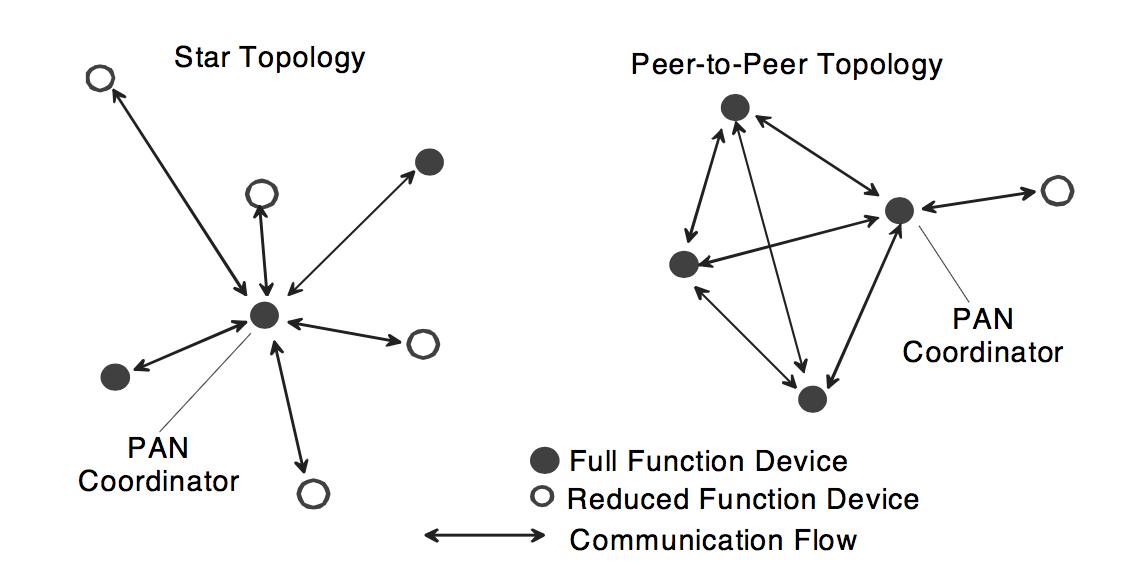
\includegraphics[scale=0.5]{Bilder/topologies}
	\caption{Topologien in IEEE 802.15.4\cite{d:ieee}}
	\label{f:topologies}
\end{figure}

Mit der Peer-to-Peer Topologie können außerdem mehrere Teilnetze zusammengefügt werden, so dass diese zu Clustern zusammengefasst werden. Ein Cluster besteht dabei aus einem PAN Coordinator sowie einigen zusätzlichen Geräten. Um clusterübergreifende Kommunikation zu ermöglichen, stellt der PAN Coordinator das Gateway in andere Cluster dar. Diese Funktion kann jedoch theoretisch jedes beliebige FFD übernehmen. Durch das Zusammenfügen mehrerer Cluster können große Netzwerke wie z.B. Sensornetze aufgebaut werden. \\
Der IEEE 802.15.4 Standard definiert selbst nur den Physical Layer und den MAC Layer, somit müssen höhere Schichten wie z.B. Vermittlung, Sicherheit und Anwendung durch weitere Technologien konkreter realisiert werden (Bsp.: ZigBee) \cite{d:hesse} \cite{d:ieee}.

\subsection{Schichten}\label{ss:Schichten}

\begin{figure}[H] 
	\centering
	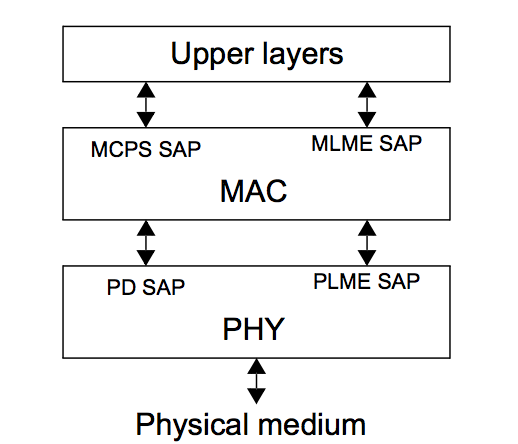
\includegraphics[scale=0.8]{Bilder/schichten}
	\caption{Definierte Schichten in IEEE 802.15.4\cite{d:ieee}}
	\label{f:schichten}
\end{figure}

IEEE 802.15.4 orientiert sich an den Schichten des ISO-OSI Referenzmodells und definiert dabei selbst nur den Physical Layer sowie den MAC Layer. \\
Die physikalische Schicht stellt die Kommunikation über so genannte ‚PHY Protocol Data Units‘ (PPDU) per Radio-Kanal bereit. Mit dem Physical Layer ist es weiterhin möglich, die Sende-Empfangseinheit zu aktivieren oder deaktivieren, Signale zu entdecken, die Qualität eines Kanals anzuzeigen und einen Kanal zu selektieren sowie zu belegen. Dies is jedoch rein auf physikalischer Ebene, die logische Belegung und Selektion erfolgt im MAC Layer.
Dieser Layer stellt das Beacon Management (s. 3.3.4) bereit, regelt den Kanalzugriff mit garantierten ‚Zeitschlitzen‘, übernimmt jegliche Fehlerbehandlung inklusive Bestätigung und realisiert gewisse sicherheitstechnische Aspekte. 802.15.4 lässt Verschlüsselung auf MAC Layer Ebene grundsätzlich zu, der dazugehörige Schlüsselaustausch findet jedoch auf darüberliegenden Schichten statt \cite{d:hesse} \cite{d:ieee}.

\subsection{Rahmenstruktur}\label{ss:Rahmenstruktur}

Durch die in der Spezifikation festgelegte Superrahmenstruktur wird die Kommunikation zwischen den Endgeräten geregelt. Dabei werden vom PAN Coordinator in gewissen Zeitabständen so genannte Beacons versendet, welche eine eindeutig Identifikationskennung des absendenden Koordinators beinhalten und unter anderem zur Netzsynchronisation und Eingliederung neuer Geräte in das Netz dienen. Der Beacon befindet sich im ersten der 16 Zeitschlitze des Superrahmens, wobei jener nicht zwingend vorhanden sein muss. Bei fehlendem Beacon wird bereits der erste Zeitschlitz zur normalen Datenübertragung genutzt. \\

\begin{figure}[H] 
	\centering
	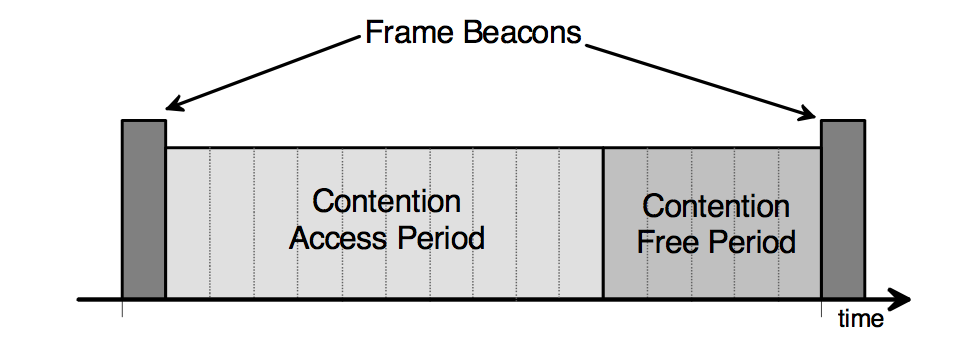
\includegraphics[scale=0.8]{Bilder/superrahmen}
	\caption{Superrahmen-Struktur eines LR-WPANs\cite{d:ieee}}
	\label{f:superrahmen}
\end{figure}

Falls nötig, kann einem Endgerät ein garantierter Zeitschlitz (‚guaranteed time slot (GTS)‘) vom PAN Coordinator zugesichert werden, in welchem es störungsfrei Daten übertragen kann. Falls diese Methode angewendet wird, findet die dazugehörige Kommunikation in der ‚Contention Free Period‘ (CFP) statt. Es findet durch die fest zugeteilten Zeitschlitze ein eindeutiger Zugriff auf das Medium statt, weswegen es in dieser Periode zu keiner Konkurrenz beim Zugriff auf das Medium kommen kann. Neben der CFP gibt es ebenfalls eine ,Contention Access Period’ (CAP), in der alle angeschlossenen Geräte unter Benutzung von CSMA/CA Daten übertragen können. Zusätzlich ist es neuen Geräten in dieser Zeit gestattet, sich in das Netzwerk zu integrieren. Falls vom PAN Coordinator keine garantierten Zeitschlitze vergeben werden, gehören alle Zeitschlitze zur CAP \cite{d:hesse} \cite{d:ieee}.

\subsection{Kommunikation}\label{ss:Kommunikation}

In der Spezifikation werden drei Arten von Kommunikationsmöglichkeiten erwähnt. Die ersten beiden Arten betreffen die Kommunikation zwischen PAN Coordinator mit einem Endgerät und umgekehrt, wobei der dritte Fall von einer direkte Kommunikation von Endgerät zu einem anderen Endgerät spricht. Der Informationsaustausch findet mit Hilfe so genannter Frames statt, von welchen wiederum vier unterschiedliche Arten existieren:

\begin{itemize}
\item Beacon Frames, welche wie oben erwähnt Informationen des PAN Coordinators enthalten
\item Data Frames, welche Daten übertragen
\item Acknowledgement Frames, welche den Empfang von anderen Frames bestätigen
\item MAC-Command Frames
\end{itemize}

\begin{figure}[H] 
	\centering
	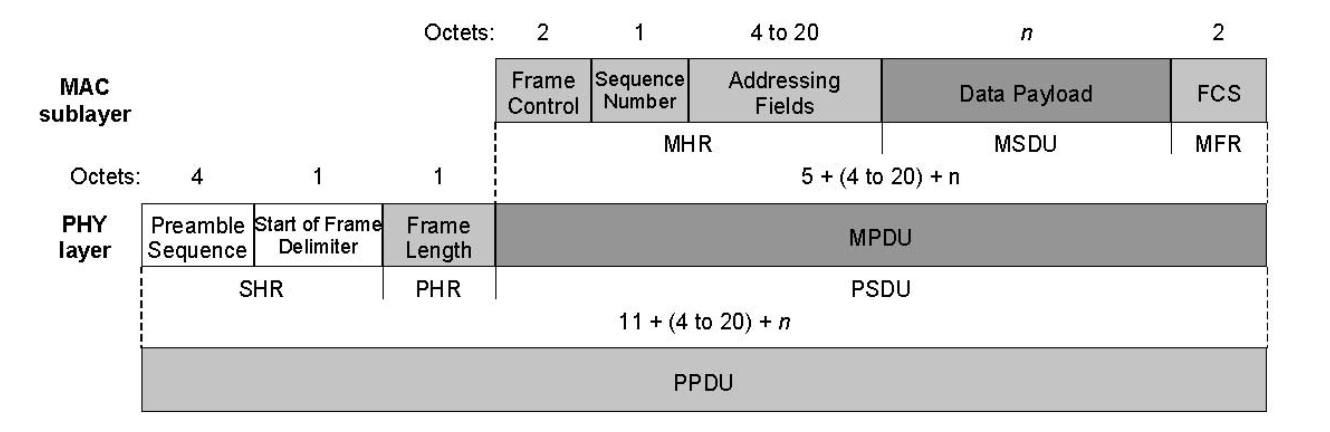
\includegraphics[scale=0.5]{Bilder/frameieee}
	\caption{Framestruktur eines Data-Frames im MAC-Layer\cite{d:ieee}}
	\label{f:frameieee}
\end{figure}

Am Anfang eines Frames steht stets ein 6 Byte-Header. Danach folgen den Anforderungen an den Frametyp entsprechend eine Packet Data Unit (PDU), welche neben einer Identifikations des Frames ebenfalls Nutzdaten beinhalten kann. Die im Frame enthaltene Payload wird in Anlehnung an das ISO/OSI-Schichtenmodell entsprechend der einzelnen Schichten gekapselt. Somit wird garantiert, dass beispielsweise der Physical Layer ausschließliche seine Header einsehen kann. Die Adressierung an andere Applikationen höherliegender Schichten ist für den Physical Layer nicht ersichtlich.
\cite{d:hesse} \cite{d:ieee}.

\subsection{Medienzugriff}\label{ss:Medienzugriff}

Ein PAN Coordinator ist nicht dazu verpflichtet, Beacons auszusenden. Die Entscheidung über die Verwendung von Beacons im Netzwerk obliegt dem Netzwerkadministrator, folglich muss der Medienzugriff der Endgeräte bei Verwendung oder Nichtverwendung gesondert betrachtet werden. \\
Falls keine Beacons zum Einsatz kommen, wird als Medienzugriffsverfahren ‚Unslotted CSMA/CA‘ benutzt. Bei diesem Verfahren wartet ein Gerät eine zufällige Zeit und überprüft nach Ablauf der Zeit den Zustand des Mediums. Sollte das Medium frei sein, wartet das Endgeräte eine weiteres Mal eine so genannte ‚Back-Off‘-Zeit ab und beginnt anschließend, bei freiem Medium seine Daten zu übertragen. Ist das Medium bereits belegt, wartet das Gerät eine weitere zufällige Zeitspanne ab, nach welcher das Medium erneut auf seinen Zustand geprüft wird.\\
Beim Einsatz von Beaconframes wird hingegen ‚Slotted CSMA/CA‘ verwendet. Das Verfahren ist dem ‚Unslotted‘-Verfahren grundsätzlich sehr ähnlich, allerdings wird die o.g. ‚Back-Off‘-Zeit so synchronisiert, dass das Gerät die Datenübertragung genau in seinem zugewiesenen Zeitschlitz beginnt und durchführt. \\
Das Versenden von Acknowledgement Frames ist im Standard definiert, ihre Benutzung ist allerdings optional. Sie werden ohne Benutzung von CSMA/CA übertragen, da sie lediglich eine Größe von 11 Byte besitzen. Innerhalb der Datenpakete kann mit Hilfe einer CRC-Prüfziffer die Integrität nach der Übertragung überprüft werden, um z.B. fehlerhafte Übertragungen zu diagnostizieren \cite{d:hesse} \cite{d:ieee}.

\subsection{Sicherheitsaspekte}\label{ss:Sicherheitsaspekte}

Im Dokument des IEEE 802.15.4 Standards werden ebenfalls einige Sicherheitsaspekte aufgelistet. Erwähnenswert ist hier die Möglichkeit, den Datentransfer auf MAC Layer-Ebene unter Verwendung von AES (‚Advanced Encryption Standard‘) zu verschlüsseln. Wie jedoch bereits erwähnt muss der Austausch der Schlüssel auf höheren Schichten stattfinden, da dieser nicht im Standard selbst definiert ist \cite{d:hesse} \cite{d:ieee}.